\section{Token economics and capacity}\label{token-economics}

Paid demand, token value, miner rewards, and operating cash are separate
quantities. Their relationship determines whether the service can expand.
This section analyzes the proposed allocation before reward caps and native
consensus effects. It assumes no future alpha price and makes no claim that
the market will finance arbitrary inference volume. Checkout, delivery, burn
finality, and refund obligations follow
Section~\ref{paid-asynchronous-jobs-and-on-chain-coordination}. The analysis
applies once the mainnet subnet's alpha exists; revenue earned before
registration accrues in the pot of Section~\ref{testnet-revenue}, whose later
purchase and burn add to the burns analyzed here.

\subsection{What customer demand changes}

For \(N_{\mathrm{job}}\) identical delivered jobs priced at
\(P_{\mathrm{USD}}=M_{\mathrm{price}} C_{\mathrm{model}}\), the principal committed to burning is
\begin{equation}\label{eq:burn-principal}
 D_{\mathrm{burn}}=N_{\mathrm{job}} M_{\mathrm{price}} C_{\mathrm{model}}.
\end{equation}
Here \(D_{\mathrm{burn}}\) is a USD valuation of customer principal, not operating revenue.
For converted payments, if \(p_{\mathrm{buy}}\) is the realized USD-equivalent
purchase price per alpha, a planning approximation is
\(B_\alpha\approx D_{\mathrm{burn}}/p_{\mathrm{buy}}\). The ledger uses actual fills and
finalized destroyed alpha. Direct alpha payments already specify the quantity
to burn and need no new market purchase. Conversion fees and any shortfall
are separately funded under the full-principal policy.

Purchases create demand where conversion is needed; burns remove alpha that
would otherwise remain in supply. The intended benefit is support for token
value, including the value held or earned by miners, validators, and owners.
This is a market hypothesis. The reduction is relative to a counterfactual
without those burns. For total alpha supply under the deployed runtime,
the stock-flow accounting is
\[
 \Delta S_\alpha=\text{gross alpha minted}-\text{all alpha burned}.
\]
Any other supply-changing runtime operation must enter that reconciliation.
Concurrent issuance can still increase supply. Burned
alpha need not exceed emissions, and a burn does not establish net deflation,
price appreciation, or immediate liquidity. Chain allocation and market
responses can change together, so the analysis does not hold aggregate
emissions constant as a protocol fact.

The multiplier \(M_{\mathrm{price}}\) controls the principal removed for a given model-cost
estimate. It therefore trades off the intended economic effect against the
price customers will accept. It supplies no cash margin to the operator or
serving miner. A usage reward separately distributes available emissions;
the customer payment creates no direct claim to a share of its proceeds.

\subsection{Rewards per unit of work}

For one accounting period, let \(E_{\mathrm{miner}}\) be the miner-emission allocation in
alpha, \(f\) its paid-use share, and \(u_i\) participant \(i\)'s verified
paid-use work units. Write \(U_{\mathrm{paid}}=\sum_i u_i>0\). The intended uncapped reward is
\begin{equation}\label{eq:usage-economics}
\begin{gathered}
 R_i^{\mathrm{use}}=f E_{\mathrm{miner}}\frac{u_i}{U_{\mathrm{paid}}},\qquad
 V_{\mathrm{pool}}=f E_{\mathrm{miner}} p,\\
 \text{USD reward per work unit}=\frac{V_{\mathrm{pool}}}{U_{\mathrm{paid}}}.
\end{gathered}
\end{equation}
The parameter \(p\) is realizable USD per alpha after sale costs at the relevant
sale size and time. It differs from the purchase price
\(p_{\mathrm{buy}}\); liquidity, slippage, and timing can separate them.
The common \(p\) is a scenario input, not a guaranteed quote available to every
participant simultaneously. \(V_{\mathrm{pool}}\) is consequently the estimated realizable
value of the paid-use pool.

Equation~\ref{eq:mechanism-allocation} reserves \(c\) for later \textit{C},
\(f\) for paid \textit{A} use, and \(1-c-f\) for \textit{A} quality.
Increasing \(f\) reallocates this budget and can weaken the quality incentive;
it does not create additional emissions. \textit{C} starts at \(c=0\), and
paid service can operate with \(f=0\). Applying this arithmetic to later
\textit{B} requires its own approved reward and native-mechanism mapping.
Native normalization, consensus, and caps can change actual payouts from
\(R_i^{\mathrm{use}}\). A zero-work usage pool, one with no paid work in its
period, has no denominator; its treatment is fixed before the pool is enabled,
never by assigning invented work.

For an approved \textit{B} paid-use pool defined analogously, write its realizable
value as \(V_{\mathrm{pool}}\) for the following capacity calculation. For
homogeneous jobs, choose one work unit per job and let
\(C_b\) be the miner's variable cost per delivered job, including its permitted
failed attempts. Then the pool's average payout is \(V_{\mathrm{pool}}/N_{\mathrm{job}}\), and variable-cost
coverage requires
\begin{equation}\label{eq:inference-capacity}
 \frac{V_{\mathrm{pool}}}{N_{\mathrm{job}}}\ge C_b,\qquad N_{\mathrm{job}}\le\frac{V_{\mathrm{pool}}}{C_b}.
\end{equation}
Here \(N_{\mathrm{job}}\) counts jobs assigned to that reward period under the finalized-burn
and fixed-lag rule. Serving costs can fall due before those rewards are realized.
This is a necessary aggregate condition under proportional allocation.
Heterogeneous costs and unequal routing can leave individual miners below
break-even. Training, fixed capacity, mandatory evaluation, and required
external reports add further costs. Quality rewards may support those costs,
but an expected award is neither guaranteed reimbursement nor cash on hand.

Public \textit{A} has a different payer: SlopNinja serves the artifact and
pays the inference bill. Rewarding its author does not reimburse that bill.
Any split between author credit and serving-cost credit must be settled before
\textit{A} calls enter a nonzero paid-use pool. The same job cannot receive
two full units merely because its author and host differ.

\subsection{Pricing sensitivity and a scale example}

The planning costs in Section~\ref{market-pricing-in-alpha} are
\(C_{\mathrm{model}}=\$0.0002875\)--\(\$0.000425\) for raw-text detection and
\(\$0.0082885\) for revision per 1,000 words. At \(M_{\mathrm{price}}=25\), their
prices are \(\$0.0071875\)--\(\$0.010625\) and \(\$0.2072125\). The \(\$0.02\)
detection target instead implies \(M_{\mathrm{price}}\approx47\)--\(70\). For a
chosen price ceiling \(P_{\mathrm{USD,max}}\), the general constraint is
\(M_{\mathrm{price}}\le P_{\mathrm{USD,max}}/C_{\mathrm{model}}\).

The comparison of raw-text detection with Pangram's dated \(\$0.40\) bulk and
\(\$0.50\) realtime rates assumes neither equivalent accuracy nor equal terms.
Subscription discounts, minimum charges, and word-block rounding still apply.

\begin{figure}[!htb]
\centering
% Planning scenarios, USD per 1,000 words; no qualified production cost.
% Raw-text launch: 1.25 * Container busy time of $0.23--$0.34 per 1,000
%   documents at 2,048 tokens (measured 2026-10-29) = .0002875--.000425.
% Later CFG profile, 8B resolver: 1.25 * (8000 * .045 + 1000 * .384) / 1e6 + .00001.
% Later CFG profile, 70B resolver: 1.25 * (20000 * .293 + 2000 * 2.253) / 1e6 + .00001.
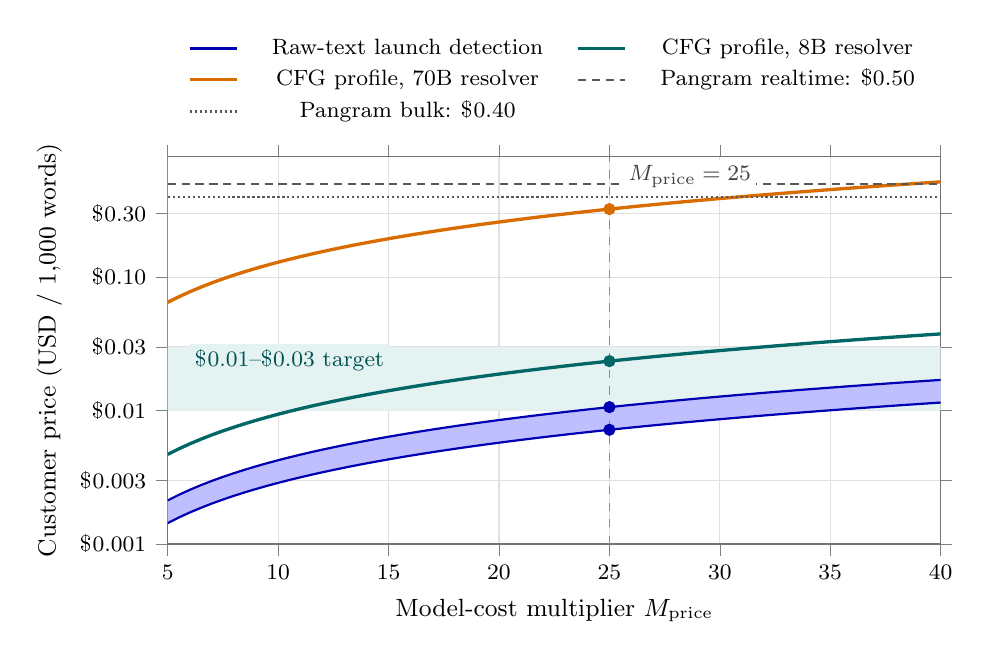
\begin{tikzpicture}
\begin{semilogyaxis}[
  width=.94\linewidth, height=6.5cm,
  xmin=5, xmax=40, ymin=.001, ymax=.8,
  xlabel={Model-cost multiplier \(M_{\mathrm{price}}\)},
  ylabel={Customer price (USD / 1,000 words)},
  xtick={5,10,15,20,25,30,35,40},
  ytick={.001,.003,.01,.03,.1,.3},
  yticklabels={\$0.001,\$0.003,\$0.01,\$0.03,\$0.10,\$0.30},
  minor y tick num=0,
  grid=major, grid style={black!12},
  tick align=outside, axis line style={black!55},
  font=\small, tick label style={font=\footnotesize},
  label style={font=\small},
  legend style={at={(.5,1.06)}, anchor=south, draw=none,
    font=\footnotesize, column sep=1em, /tikz/every even column/.append style={column sep=1em}},
  legend columns=2,
  clip=true,
]
\addplot[draw=none, fill=teal!10, forget plot]
  coordinates {(5,.01) (40,.01) (40,.03) (5,.03)} \closedcycle;
\addplot[draw=none, fill=blue!25, forget plot]
  coordinates {(5,0.0014375) (7.5,0.00215625) (10,0.002875) (12.5,0.00359375) (15,0.0043125) (17.5,0.00503125) (20,0.00575) (22.5,0.00646875) (25,0.0071875) (27.5,0.00790625) (30,0.008625) (32.5,0.00934375) (35,0.0100625) (37.5,0.01078125) (40,0.0115)
    (40,0.017) (37.5,0.0159375) (35,0.014875) (32.5,0.0138125) (30,0.01275) (27.5,0.0116875) (25,0.010625) (22.5,0.0095625) (20,0.0085) (17.5,0.0074375) (15,0.006375) (12.5,0.0053125) (10,0.00425) (7.5,0.0031875) (5,0.002125)} \closedcycle;
\addplot[blue!70!black, thick, domain=5:40, samples=71] {.000425*x};
\addlegendentry{Raw-text launch detection}
\addplot[blue!70!black, thick, domain=5:40, samples=71, forget plot] {.0002875*x};
\addplot[teal!80!black, very thick, domain=5:40, samples=71] {.00094*x};
\addlegendentry{CFG profile, 8B resolver}
\addplot[orange!85!black, very thick, domain=5:40, samples=71] {.0129675*x};
\addlegendentry{CFG profile, 70B resolver}
\addplot[black!65, densely dashed, thick] coordinates {(5,.50) (40,.50)};
\addlegendentry{Pangram realtime: \$0.50}
\addplot[black!65, densely dotted, thick] coordinates {(5,.40) (40,.40)};
\addlegendentry{Pangram bulk: \$0.40}
\addplot[black!45, dashed, forget plot] coordinates {(25,.001) (25,.8)};
\addplot[only marks, mark=*, mark size=2pt, blue!70!black, forget plot]
  coordinates {(25,.0071875) (25,.010625)};
\addplot[only marks, mark=*, mark size=2pt, teal!80!black, forget plot]
  coordinates {(25,.0235)};
\addplot[only marks, mark=*, mark size=2pt, orange!85!black, forget plot]
  coordinates {(25,.3241875)};
\node[anchor=north west, font=\footnotesize, text=black!75,
  fill=white, inner sep=2pt] at (axis cs:25.6,.76) {\(M_{\mathrm{price}}=25\)};
\node[anchor=west, font=\footnotesize, text=teal!65!black,
  fill=teal!10, inner sep=2pt] at (axis cs:6,.024) {\$0.01--\$0.03 target};
\end{semilogyaxis}
\end{tikzpicture}

\caption{Price sensitivity per 1,000-word detection job. The band spans the
raw-text cost of \$0.0002875--\$0.000425 from measured Container busy time,
including the stated retry allowance. The shaded \$0.01--\$0.03 range is the
proposed detection target; Pangram's dated bulk and realtime rates are price
comparisons only. The price axis is logarithmic. No token-price assumption
enters this calculation.}
\label{fig:pricing-sensitivity}
\end{figure}

The revision scenario assigns \(\$0.00271875\) per job to the miner's proposer
calls. Operator model, compute, storage, and delivery costs are approximately
\(\$0.0079\)--\(\$0.0085\). Raw-text detection's corresponding operator subtotal
is \(\$0.0004\)--\(\$0.0009\). Table~\ref{tab:tokenomics-volume} scales these
proxies without economies of scale. Burn principal is unavailable for either
party's bills.

Revision cost is sensitive to its resolver. The batched 8B resolution budget
costs \(\$0.00093\) after the retry allowance; a 70B resolver using 20,000 input
and 2,000 output tokens at the stated tariff would cost \(\$0.0129575\) instead,
raising revision model cost from \(\$0.0082885\) to \(\$0.020316\), about
\(\$0.5079\) at \(M_{\mathrm{price}}=25\). For such workloads the escalation
rate and workload bounds matter more than the multiplier.

\begin{table}[htbp]
\centering\small
\begin{tabularx}{\linewidth}{Lrrrr}
\toprule
Service & Jobs & Burn principal & Miner serving & Operator delivery \\
\midrule
Detection & 1,000 & \$7.19--\$10.63 & --- & \$0.39--\$0.93 \\
Detection & 100,000 & \$719--\$1,063 & --- & \$39--\$93 \\
Revision & 1,000 & \$207.21 & \$2.72 & \$7.90--\$8.50 \\
Revision & 100,000 & \$20,721.25 & \$271.88 & \$790--\$850 \\
\bottomrule
\end{tabularx}
\caption{Illustrative period totals at \(M_{\mathrm{price}}=25\) for 1,000-word jobs, rounded
for display. Serving costs use tariff proxies, the synthetic-text Container
measurement, and assumed retry/runtime budgets, not production measurements. They exclude payment and chain fees,
refund reserves, training, evaluation, external checks, and low-volume fixed
costs. Public \textit{A} has no miner serving charge in this architecture.}
\label{tab:tokenomics-volume}
\end{table}

\subsection{Capacity and operating reserves}

If volume grows by a factor \(k\) while per-job cost stays unchanged, \(V_{\mathrm{pool}}\)
must also grow by at least \(k\) to preserve the same reward per job. The average
log elasticity over that change must therefore be at least one.
Purchase-and-burn establishes no law forcing this response:
\(f\), \(E_{\mathrm{miner}}\), and realizable \(p\) may each remain flat or fall. With a fixed
pool, doubling volume halves the reward per unit. Equation~\ref{eq:inference-capacity}
then gives a budget-dependent serving limit, not unlimited scalability.

\begin{figure}[htbp]
\centering
% Homogeneous bounded-revision planning scenario. Each job is 1,000 words.
% Cash costs and burned principal are distinct flows, all expressed in USD.
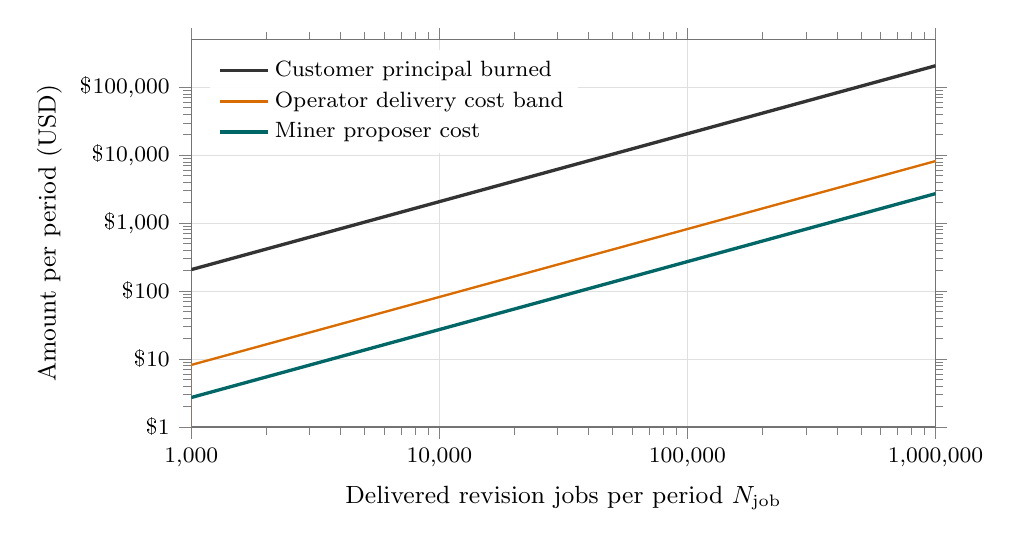
\begin{tikzpicture}
\begin{loglogaxis}[
  width=.91\linewidth, height=6.5cm,
  xmin=1000, xmax=1000000, ymin=1, ymax=500000,
  xlabel={Delivered revision jobs per period \(N_{\mathrm{job}}\)},
  ylabel={Amount per period (USD)},
  xtick={1000,10000,100000,1000000},
  xticklabels={{1,000},{10,000},{100,000},{1,000,000}},
  ytick={1,10,100,1000,10000,100000},
  yticklabels={\$1,\$10,\$100,{\$1,000},{\$10,000},{\$100,000}},
  minor x tick num=0, minor y tick num=0,
  grid=major, grid style={black!12},
  tick align=outside, axis line style={black!55},
  font=\small, tick label style={font=\footnotesize},
  label style={font=\small},
  legend style={at={(.025,.975)}, anchor=north west, draw=none,
    fill=white, fill opacity=.95, text opacity=1, font=\footnotesize,
    cells={anchor=west}},
  clip=true,
]
\addplot[black!80, very thick, domain=1000:1000000, samples=2] {.2072125*x};
\addlegendentry{Customer principal burned}
\addplot[draw=none, fill=orange!60, forget plot]
  coordinates {(1000,7.9) (1000000,7900) (1000000,8500) (1000,8.5)} \closedcycle;
\addplot[orange!85!black, thick, domain=1000:1000000, samples=2] {.0082*x};
\addlegendentry{Operator delivery cost band}
\addplot[teal!80!black, very thick, domain=1000:1000000, samples=2] {.00271875*x};
\addlegendentry{Miner proposer cost}
\end{loglogaxis}
\end{tikzpicture}

\caption{Revision totals versus delivered 1,000-word jobs in one period.
Burn principal is \$0.2072125 per job; miner proposer cost is \$0.00271875;
operator delivery costs span \$0.0079--\$0.0085. Both axes are logarithmic.
The curves scale fixed planning assumptions and exclude the additional costs
listed in Table~\ref{tab:tokenomics-volume}. The burn curve is not a funding
source, and no alpha price or emission trajectory is forecast.}
\label{fig:volume-sensitivity}
\end{figure}

Operator solvency needs its own constraint. Let \(T_{\mathrm{cash}}\) be available treasury
cash excluding customer custody, \(F_{\mathrm{cash}}\) additional realized operating funding,
\(O_{\mathrm{due}}\) service and shared expenses due, \(L_{\mathrm{due}}\) refunds and other liabilities
due, and \(H_{\mathrm{reserve}}\) the required reserve for remaining future obligations. Admission
must preserve
\[
 T_{\mathrm{cash}}+F_{\mathrm{cash}}-O_{\mathrm{due}}-L_{\mathrm{due}}\ge H_{\mathrm{reserve}}.
\]
No term includes burned principal. Capital or explicitly allocated, realized
owner proceeds can contribute to \(F_{\mathrm{cash}}\); future emissions cannot. Native owner
entitlement follows the ownership or lease arrangement and does not itself
entitle SlopNinja or an investor to those proceeds. Reserves must also match
the currencies and timing of liabilities, so a USD-equivalent surplus alone
does not establish that refunds can be paid.

\subsection{Self-purchases and low-volume rewards}

Burning gives artificial demand a cost, but a large pool divided among little
legitimate work can still reward it. Let \(U_{\mathrm{honest}}>0\) be existing legitimate
work, \(u_{\mathrm{self}}\) additional self-purchased work credited to an attacker, and \(k_s\)
the attacker's incremental cost per such unit, including the full customer
price and its own variable serving costs. For an attacker with no preexisting
share, holding \(V_{\mathrm{pool}}\) fixed gives the simplified gain
\begin{equation}\label{eq:self-purchase-gain}
 \Pi(u_{\mathrm{self}})=V_{\mathrm{pool}}\frac{u_{\mathrm{self}}}{U_{\mathrm{honest}}+u_{\mathrm{self}}}-k_s u_{\mathrm{self}}.
\end{equation}
This assumes the attacker can route the purchases to its own credited model.
If it already earns \(V_{\mathrm{pool}} u_a/U_{\mathrm{honest}}\) from legitimate work, measure incremental
gain instead:
\[
 \Delta\Pi(u_{\mathrm{self}})=V_{\mathrm{pool}}\left(\frac{u_a+u_{\mathrm{self}}}{U_{\mathrm{honest}}+u_{\mathrm{self}}}-\frac{u_a}{U_{\mathrm{honest}}}\right)-k_s u_{\mathrm{self}}.
\]
Existing rewards are not new attack proceeds. Both expressions omit caps,
price feedback, quality-reward changes, and other controlled identities.

\begin{figure}[htbp]
\centering
% Hypothetical fixed reward pool V_{\mathrm{pool}}, honest work U_{\mathrm{honest}} > 0, no prior attacker work.
% r_self = u_self / U_honest; a = full self-purchase cost per work * U_honest / V_pool.
% Normalized incremental payoff is r_self/(1+r_self) - a*r_self.
% PGFPlots' internal variable x represents r_self. No token-price forecast.
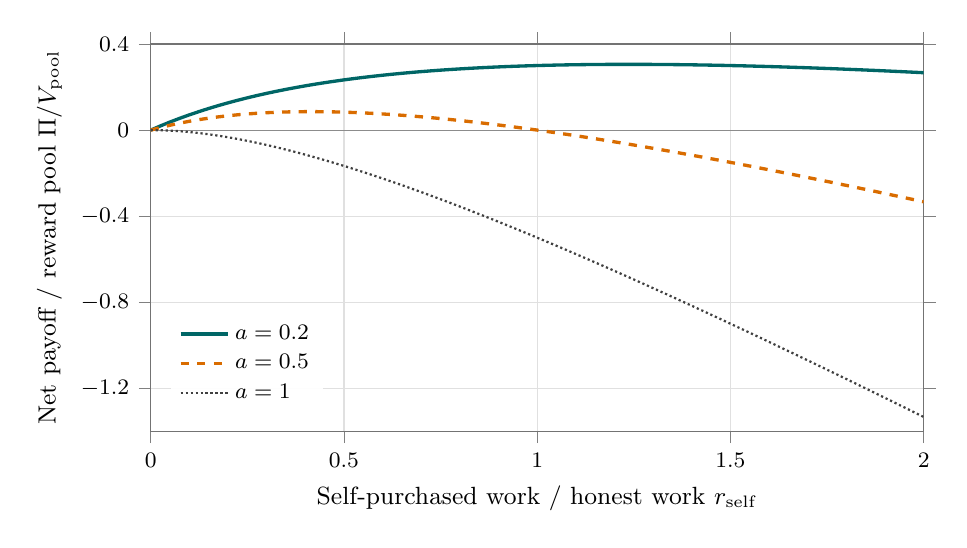
\begin{tikzpicture}
\begin{axis}[
  width=.94\linewidth, height=6.5cm,
  xmin=0, xmax=2, ymin=-1.4, ymax=.4,
  xlabel={Self-purchased work / honest work \(r_{\mathrm{self}}\)},
  ylabel={Net payoff / reward pool \(\Pi/V_{\mathrm{pool}}\)},
  xtick={0,.5,1,1.5,2},
  ytick={-1.2,-.8,-.4,0,.4},
  grid=major, grid style={black!12},
  tick align=outside, axis line style={black!55},
  font=\small, tick label style={font=\footnotesize},
  label style={font=\small},
  legend style={at={(.025,.045)}, anchor=south west, draw=none,
    fill=white, fill opacity=.95, text opacity=1, font=\footnotesize,
    cells={anchor=west}},
  clip=true,
]
\addplot[black!45, thin, forget plot] coordinates {(0,0) (2,0)};
\addplot[teal!80!black, very thick, domain=0:2, samples=81] {x/(1+x)-.2*x};
\addlegendentry{\(a=0.2\)}
\addplot[orange!85!black, very thick, dashed, domain=0:2, samples=81] {x/(1+x)-.5*x};
\addlegendentry{\(a=0.5\)}
\addplot[black!75, thick, densely dotted, domain=0:2, samples=81] {x/(1+x)-x};
\addlegendentry{\(a=1\)}
\end{axis}
\end{tikzpicture}

\caption{Simplified self-purchase incentive with fixed \(V_{\mathrm{pool}}>0\), honest
traffic \(U_{\mathrm{honest}}>0\), no preexisting attacker credit, and no reward cap. Set
\(r_{\mathrm{self}}=u_{\mathrm{self}}/U_{\mathrm{honest}}\) and \(a=k_s U_{\mathrm{honest}}/V_{\mathrm{pool}}\); normalized gain is
\(\Pi/V_{\mathrm{pool}}=r_{\mathrm{self}}/(1+r_{\mathrm{self}})-a r_{\mathrm{self}}\). Curves vary the cost of buying work relative to the
pool. They are sensitivity cases, not measured attack profitability.}
\label{fig:self-purchase-sensitivity}
\end{figure}

With no preexisting attacker credit, the initial marginal gain is positive
when \(V_{\mathrm{pool}}/U_{\mathrm{honest}}>k_s\). With no honest
work, any positive sole credited purchase can capture the entire uncapped
pool. A cap on work units or on one identity's share does not solve this after
renormalization or identity splitting. Qualification needs an absolute cap on
released rewards relative to attributable paid burn, applied across common
control and the total pool, with an explicit destination for unused allocation.
No numerical cap or implementation is selected here. Validator dividends,
owner proceeds, and other rewards under common control must enter the combined
attack budget; a miner-only calculation cannot establish resistance.

\subsection{Calibration and activation decisions}

Low demand makes reward concentration and fixed costs more important; high
demand raises aggregate bills and can dilute rewards below serving cost.
Calibration must test both regimes, including declining realizable token value,
illiquid sales, resolver escalation in later \textit{B}'s parsed workloads, retry spikes, provider repricing,
delayed burns, and post-burn refunds. Use measured cost distributions rather
than only averages, and treat free beta inference as a temporary subsidy.

Before enabling a paid-use pool, fix workload credit, author-versus-serving
credit, \(f\), release caps, zero-work pool treatment, and the native payout mapping.
Choose \(M_{\mathrm{price}}\) against measured quality, customer prices, and operating capacity;
fund reserves before accepting liabilities. Update offers and future reward
schedules through their published versioning rules. Rising burns or demand
alone do not justify raising capacity beyond funded obligations and miners'
willingness to serve.
